\documentclass[a4paper]{article}
\usepackage[utf8]{inputenc}
\usepackage[fleqn]{amsmath}
\usepackage{amssymb}
\usepackage{mathtools}
\usepackage{amsfonts}
\usepackage{lastpage}
\usepackage{tikz}
\usepackage{float}
\usepackage{textcomp}
\usetikzlibrary{patterns}
\usepackage{pdfpages}
\usepackage{gauss}
\usepackage{fancyvrb}
\usepackage[table]{colortbl}
\usepackage{fancyhdr}
\usepackage{graphicx}
\usepackage[margin=2.5 cm]{geometry}

\definecolor{listinggray}{gray}{0.9}
\usepackage{listings}
\lstset{
    language=,
    literate=
        {æ}{{\ae}}1
        {ø}{{\o}}1
        {å}{{\aa}}1
        {Æ}{{\AE}}1
        {Ø}{{\O}}1
        {Å}{{\AA}}1,
    backgroundcolor=\color{listinggray},
    tabsize=3,
    rulecolor=,
    basicstyle=\scriptsize,
    upquote=true,
    aboveskip={0.2\baselineskip},
    columns=fixed,
    showstringspaces=false,
    extendedchars=true,
    breaklines=true,
    prebreak =\raisebox{0ex}[0ex][0ex]{\ensuremath{\hookleftarrow}},
    frame=single,
    showtabs=false,
    showspaces=false,
    showlines=true,
    showstringspaces=false,
    identifierstyle=\ttfamily,
    keywordstyle=\color[rgb]{0,0,1},
    commentstyle=\color[rgb]{0.133,0.545,0.133},
    stringstyle=\color[rgb]{0.627,0.126,0.941},
  moredelim=**[is][\color{blue}]{@}{@},
}

\lstdefinestyle{base}{
  emptylines=1,
  breaklines=true,
  basicstyle=\ttfamily\color{black},
}

\pagestyle{fancy}
\def\checkmark{\tikz\fill[scale=0.4](0,.35) -- (.25,0) -- (1,.7) -- (.25,.15) -- cycle;}
\newcommand*\circled[1]{\tikz[baseline=(char.base)]{
            \node[shape=circle,draw,inner sep=2pt] (char) {#1};}}
\newcommand*\squared[1]{%
  \tikz[baseline=(R.base)]\node[draw,rectangle,inner sep=0.5pt](R) {#1};\!}
\newcommand{\comment}[1]{%
  \text{\phantom{(#1)}} \tag{#1}}
\cfoot{Page \thepage\ of \pageref{LastPage}}
\DeclareGraphicsExtensions{.pdf,.png,.jpg}
\author{Nikolaj Dybdahl Rathcke (rfq695) \\ Victor Petrèn Bach Hansen (grn762)}
\title{Advanced Computer Systems \\ Assignment 2}
\lhead{Advanced Computer System}
\rhead{Assignment 2}

\begin{document}
\maketitle

\section{Serializability \& Locking}

\subsection{}
The precedence graph for schedule $1$ is:
\begin{center}
    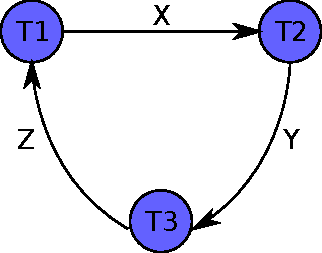
\includegraphics{fig1}
\end{center}
This means the schedule is not conflict-serializable as the graph contains a cycle. The letters indicate on what object there is a potential conflict. The graphs shows that T1 must run before T2, otherwise there is a conflict with object $X$. Likewise T2 must run before T3 and T3 before T1 to avoid conflicts. This is not possible. \\
\\
The precedence graph for schedule $2$ is:
\begin{center}
    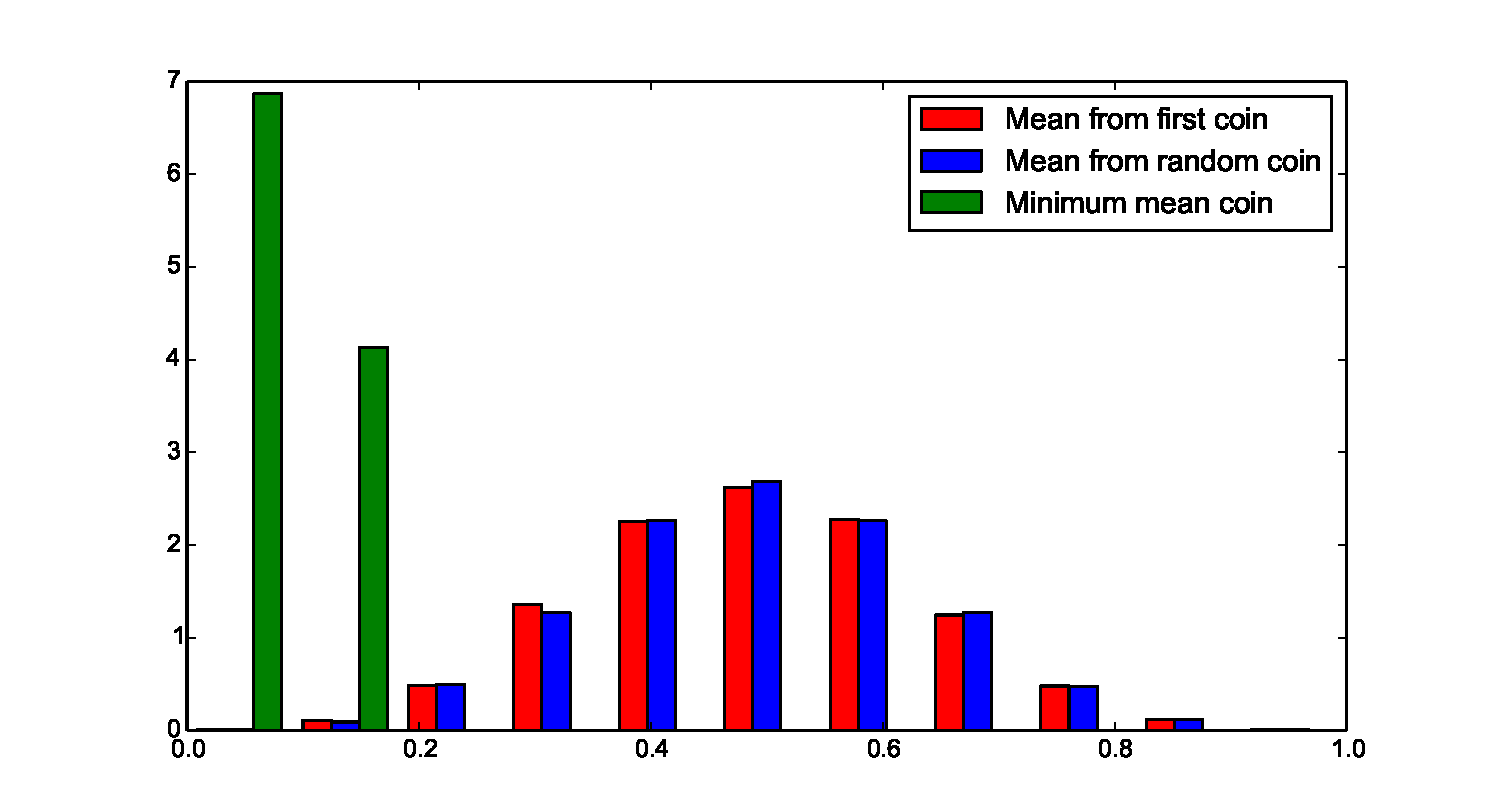
\includegraphics{fig2}
\end{center}
This schedule is conflict serializable. There is not cycle. T1 and T3 has nothing to do with each other, so as long as we run T2 last, there is not problem. We can actually run it in order \{T1, T3, T2\} and \{T3, T1, T2\} and there will be no conflicts.

\subsection{}
Let $S(X)$ denote we make a shared lock on $X$, $E(X)$ denote we make an exclusive lock on $X$ and $R(X)$ denote we release the locks (this happens when there is a commit). \\
For schedule $1$, we would get the following lock operation:
\begin{verbatim}
    T1: S(X)    E(Y)R(X)R(Y)
    T2:     E(Z)            E(X)R(Z)R(X)
    T3:                                 S(Z)S(Y)R(Z)R(Y)
\end{verbatim}
So no, it can not be scheduled with strict 2PL as T3 ends up reading object Y that has been modified by T1. \\
\\
The lock operation for schedule $2$ would look like:
\begin{verbatim}
    T1: S(X)            E(Y)R(X)R(Y)
    T2:             S(Z)            E(X)E(Y)R(Z)R(X)R(Y)
    T3:     E(Z)R(Z)
\end{verbatim}
This can be scheduled with strict 2PL as there are no conflicts.

\section{Optimistic Concurrency Control}

\subsection{Scenario 1}
There is no conflicts between \texttt{T1} and \texttt{T3} since \texttt{T1} completes and commits its changes before \texttt{T3} starts. There is, however, a conflict between \texttt{T2} and \texttt{T3}. As $\texttt{WriteSet(T2)} \cap \texttt{ReadSet(T3)}$ is not an empty set, since \texttt{T3} reads from \texttt{3} before \texttt{T2} writes to it, \texttt{T3} will read dirty data. Thus \texttt{T3} will have to roll back.
\subsection{Scenario 2}
In this scenario, we have a conflict between \texttt{T1} and \texttt{T3}. Because $\texttt{WriteSet(T1)} \cap \texttt{ReadSet(T3)}$ is not an empty set, since \texttt{T3} reads from \texttt{3} before \texttt{T1} writes to it, \texttt{T3} will read dirty data. Thus \texttt{T3} will have to roll back.

There is no conflict between \texttt{T2} and \texttt{T3} since $\texttt{WriteSet(T2)} \cap \texttt{ReadSet(T3)} = \varnothing$ and $\texttt{WriteSet(T2)} \cap \texttt{WriteSet(T3)} = \varnothing$.
\subsection{Scenario 3}
There are no conflicts between either \texttt{T1} and \texttt{T3} or \texttt{T2} and \texttt{T3}. This is because both \texttt{T1} and \texttt{T2} both finishes their write phases before \texttt{T3} where $\texttt{WriteSet(T1)} \cap \texttt{ReadSet(T3)} = \varnothing$ and $\texttt{WriteSet(T2)} \cap \texttt{ReadSet(T3)} = \varnothing$. \texttt{T3} can therefore commit its changes.

\section{Programming Task}
The implemented code is performed only in the \texttt{ConcurrentCertainBookStore} class. The tests are all implemented in the class \texttt{ConcurrentTest}. The entire source code for the bookstore is found in the \texttt{acertainbookstore-2015.2.1/src} folder.

\section{Discussion on the Concurrent Implementation of Bookstore}
\subsection{}
The implementation uses the strategy of locking the books we are working on. Namely, we lock on their ISBN. The implementation lock all the books before reading or writing and unlocks them afterwards to achieve before-or-after atomicity. We make use of the \texttt{try-finally} syntax to ensure the unlocking phase happens even if something goes wrong in the reading/writing phase. The locks are stored in a concurrent hashmap with the ISBN as keys and the lock as values. The only time we add a new
ISBN to the map (a key) is when we call \texttt{addBooks}, in which case we create a new entry in the hashmap .

To protect the \texttt{bookMap}, we also utlize a global lock when we require to look at the \texttt{bookMap} as a whole, such as \texttt{getBooks()} or \texttt{listEditorPicks(int numBooks)}, or when we are performing an operation which resizes the \texttt{bookMap}, such as when adding or removing books. This is done to avoid getting dirty reads, e.g. attempting to remove a key from the map while at the same time attempting to get all the books contained in it.
\\ \\
To test concurrency and lock management, we implemented $4$ tests, shown below. Each test starts 2 new client-threads, which is implemented in each their own seperate class that extends \texttt{Thread}. The \texttt{run} method in each of these client-thread classes then implements the works described in the various test cases.
\begin{enumerate}
\item First test, called \texttt{testConcurrentBuyAndRestock}, works by a thread $C1$ and a thread $C2$ calling \texttt{buyBooks} and \texttt{addCopies} respectively. They call the methods with the same set of books, and since they each method is called the same number of times, we should end up with the same number of books (for each ISBN) as we started with. If this is verified, it means the operations do not have conflicting writes.
\item The test \texttt{testBuyRestockConsistentSnapshot} tests that when a thread $C1$ buys a collection of books ($2$ copies of a book with ISBN $5$), and then restock the same collection will mean that when another thread $C2$ invoke \texttt{getBooks}, that call returns either a snapshot of when we just bought or just restocked. Since we start with $5$ copies of the book, we should have either $3$ or $5$ copies. This ensures we do not have any dirty reads.
\item The test \texttt{testNoDeadlocks} tests that when two threads buys the same collection of books (but in reverse order), they do not deadlock since we sort by ISBN before acquiring locks. The two threads also restock the same collection of books and we ensure there are the same amount of books as we started with - again showing there are no dirty writes.
\item The last test, \texttt{testConcurrentRemoveRestockAndGetBooksByISBN}, a bit similar to the second test, checks that when a thread removes a book by its ISBN and restock it afterwards, another thread will either see that the book does not exist or that it has the same amount as we started with. If this is verified, we do not have any dirty reads with these methods.
\end{enumerate}
The test all succeed (also when running them many times) indicating that our locking implementation works as intended.

\subsection{}
The locking we are using is essentially conservative strict 2PL. We lock everything before doing anything and release them all when we are done. This means we have less concurrency than the other flavours of 2PL locking schemes, but we avoid deadlocks and cascading aborts.

\subsection{}
Since it is a conservative strict 2PL we have implemented, we should not get any deadlocks. This is because we also sort the ISBN's before trying to acquire the locks, so if two threads are trying to acquire the same locks, they will try to acquire them in the same order and as such, one of them must be able to get all the locks it need.

\subsection{}
Since the thread-safe method calls require us to lock the resources we are working with, one bottleneck is we can only handle a finite amount of requests at the same time, as otherwise some would have to wait for the locks to be unlocked. This means we can end up with a queue of clients waiting to be served which immediately is not a problem, but since a connection can time out, this actually means we can not infinitely scale the number of clients.


Even though we use a locking strategy that provides less concurrency that the other 2PL variants, we will have some performance improvement. Obviously, if we have very few books, we lose almost the same as the overhead being paid. But if we can assume our bookstore is reasonable large, we will gain something. \\
To make a \textbf{very} rough estimate, we can typically say a normal method call iterates through a set of books and does some work that is usually constant times. A thread-safe method call also takes time unlocking and locking the same amount of books. A thread-safe methods call also has some overhead when creating threads and coordination work going into it. Lets disregard that sometimes two threads are waiting for each other anyways because they are accessing the same resource, and we say a method call takes $t$ time (without respecting concurrency).

Lets say a thread-safe method call takes $m\cdot t$ time (a normal method call takes $t$ time). Now if we want to handle $n$ request, without concurrency, we can estimate this takes $n\cdot t$ time. With concurrency, if we can serve $m+1$ people, we will have a higher throughput. We can fairly say that, if our bookstore is a reasonable size, since $m$ is not very large and we can expect $n>m$ (if our bookstore is just somewhat popular).

\end{document}
